% -*- latex -*-
%
% The SAND document class is maintained at:
%
%    http://www.cs.sandia.gov/SANDreport
%
% This page also has instructions and documentation on commands.
%
\documentclass[12pt,report]{SANDreport}

\SANDnum{SAND20XX-XXXX}
\SANDprintDate{January 20XX}

\title{VTK-m Users' Guide \\
  \relsize{-2}Version 0.0
}
\author{Kenneth~Moreland \\
  \relsize{-2} Scalable Analysis and Visualization \\[-1ex]
  \relsize{-2} Sandia National Laboratories \\[-1ex]
  \relsize{-2} P.O. Box 5800 MS 1323 \\[-1ex]
  \relsize{-2} Albuquerque, NM 87185-1323 \\[-1ex]
  \relsize{-2} kmorel@sandia.gov
}
\SANDauthor{Kenneth~Moreland}
\date{} % Leave empty


\usepackage{amsfonts}
\usepackage{amssymb}
\usepackage{amsmath}
\usepackage{booktabs}
\usepackage{graphicx}
\usepackage{isomath}
\usepackage{varioref}
\usepackage{fancyvrb}
\usepackage{ifthen}
\usepackage{longtable}
\usepackage{cite}
\usepackage{relsize}
\usepackage{subfig}
\usepackage{xspace}

% This wonderful package allows hyphenation in tt fonts and hyphenation of
% words with underscores in them.
\usepackage[htt]{hyphenat}

% This package defines a tt font that supports boldface (albeit not very
% distinctly). The default package has no boldface for tt fonts.
\usepackage{lmodern}

\usepackage{makeidx}
\makeindex

\usepackage[pdfborder={0 0 0}]{hyperref}
\usepackage{verbatim}

\usepackage{color}
\definecolor{yellow}{rgb}{1,1,0}
\definecolor{black}{rgb}{0,0,0}
\definecolor{ltcyan}{rgb}{.75,1,1}
\definecolor{red}{rgb}{1,0,0}
\definecolor{gray}{rgb}{.6,.6,.6}
\definecolor{darkred}{rgb}{0.5,0,0}
\definecolor{darkgreen}{rgb}{0,0.5,0}

\definecolor{vtkmidentifier}{rgb}{0,0,1}
\definecolor{vtkmnamespace}{rgb}{0.5,0,0}
\definecolor{vtkmmacro}{rgb}{0.5,0,0}
\definecolor{vtkmsignature}{rgb}{0,0.5,0}

\usepackage{listings}
\lstloadlanguages{C,C++}
\lstset{fontadjust=false,basicstyle=\scriptsize\ttfamily}
%% \lstset{numbers=left, numberstyle=\tiny, stepnumber=1, numbersep=2pt}
\lstdefinelanguage{VTKm}{
  morekeywords={struct,class,public,typedef,void,template,return,operator,const,for,int},
  morekeywords={[2]Id,Id2,Id3,Scalar,Tuple,Vector2,Vector3,Vector4,
                   make_Id3,make_Vector2,make_Vector3,make_Vector4,
                   dot,NUM_COMPONENTS,
                   Extent,Extent3,Pair,
                   ExtentPointDimensions,ExtentCellDimensions,
                   ExtentNumberOfPoints,ExtentNumberOfCells,
                   ExtentPointFlatIndexToTopologyIndex,
                   ExtentCellFlatIndexToTopologyIndex,
                   ExtentPointTopologyIndexToFlatIndex,
                   ExtentCellTopologyIndexToFlatIndex,
                   WorkletMapField, WorkletMapCell,
                   WorkletGenerateTopology, WorkletInterpolatedCell,
                   WorkletGenerateKeysValues, WorkletReduceKeysValues,
                   ExecutionObjectBase,
                   TypeTraits,NumericTag,DimensionalityTag,
                   TypeTraitsRealTag,TypeTraitsIntegerTag,
                   TypeTraitsScalarTag,TypeTraitsVectorTag,
                   VectorTraits,ComponentType,HasMultipleComponents,
                   VectorTraitsTagMultipleComponents,
                   VectorTraitsTagSingleComponent,
                   Error, ErrorExecution, ErrorControl,
                   ErrorControlAssert, ErrorControlBadValue,
                   ErrorControlInternal, ErrorControlOutOfMemory,
                   DeviceAdapterTagSerial,
                   DeviceAdapterTagCuda,
                   DeviceAdapterTagOpenMP,
                   DeviceAdapterTagTBB,
                   CellAverage,
                   CellDataToPointDataGenerateKeys,CellDataToPointDataReduceKeys,
                   CellGradient,
                   Cosine,Sine,Magnitude,Square,
                   Elevation,
                   MarchingCubesClassify,MarchingCubesGenerate,
                   PointDataToCellData,
                   SliceClassify,SliceGenerate,
                   Tetrahedralize,
                   ThresholdClassify,ThresholdTopology,
                   ArrayHandle,make_ArrayHandle,
                   ArrayHandleConstant,make_ArrayHandleConstant,
                   ArrayHandleCounting,make_ArrayHandleCounting,
                   ArrayContainerControl,
                   ArrayContainerControlTagBasic,
                   ArrayContainerControlTagImplicit,
                   ArrayTransfer,
                   ArrayManagerExecution,
                   ArrayManagerExecutionShareWithControl,
                   DeviceAdapterAlgorithm, DeviceAdapterAlgorithmGeneral,
                   IteratorFromArrayPortal,
                   UniformGrid,UnstructuredGrid,
                   DispatcherMapField, DispatcherMapCell,
                   DispatcherGenerateTopology, DispatcherInterpolatedCell,
                   DispatcherGenerateKeysValues,
                   DispatcherReduceKeysValues,
                   CellField, CellVertices,
                   InterpolatedCellPoints,
                   CellTraits,NUM_VERTICES,
                   CellTagHexahedron, CellTagLine, CellTagQuadrilateral,
                   CellTagTetrahedron, CellTagTriangle, CellTagVectex,
                   CellTagVoxel, CellTagWedge,
                   CellTraits,
                   CellTopologicalDimensionsTag,
                   GridTagUniform, GridTagUnstructured,
                   NUM_VERTICES, TOPOLOGICAL_DIMENSIONS,
                   ParametricCoordinates, CellDerivative,
                   SortLess, SortGreater,
                   Max, Min,
                   Cbrt, Exp, Exp10, Exp2, ExpM1, Log, Log10, Log1P, Log2,
                   Pow, RCbrt, RSqrt, Sqrt,
                   Matrix, Matrix2x2, Matrix3x3, Matrix4x4,
                   MatrixColumn, MatrixDeterminant, MatrixIdentity,
                   MatrixInverse, MatrixMultiply, MatrixRow,
                   MatrixSetColumn, MatrixSetRow, MatrixTranspose,
                   SolveLinearSystem,
                   NewtonsMethod,
                   Ceil, Epsilon, Floor, FMod, Infinity, IsFinite, IsInf,
                   IsNan, ModF, Nan, NegativeInfinity, Remainder,
                   RemainderQuotient, Round,
                   Abs, CopySign, IsNegative, SignBit,
                   ACos, ACosH, ASin, ASinH, ATan, ATan2, ATanH, Cos, CosH,
                   Pi, Sin, SinH, Tan, TanH,
                   Cross, Magnitude, MagnitudeSquared, Lerp, Normal,
                   Normalize, RMagnitude, TriangleNormal,
                   ParametricCoordinatesToWorldCoordinates,
                   WorldCoordinatesToParametricCoordinates,
                   ParametricCoordinates,
                   TransferToOpenGL
                   },
  morekeywords={[3]VTKM_CONT_EXPORT,VTKM_EXEC_EXPORT,VTKM_EXEC_CONT_EXPORT,
                   VTKM_EXEC_CONSTANT_EXPORT,
                   VTKM_DEVICE_ADAPTER,
                   VTKM_DEVICE_ADAPTER_SERIAL,
                   VTKM_DEVICE_ADAPTER_CUDA,
                   VTKM_DEVICE_ADAPTER_OPENMP,
                   VTKM_DEVICE_ADAPTER_TBB,
                   VTKM_DEVICE_ADAPTER_ERROR,
                   VTKM_DEFAULT_DEVICE_ADAPTER_TAG,
                   VTKM_ARRAY_CONTAINER_CONTROL,
                   VTKM_ARRAY_CONTAINER_CONTROL_BASIC,
                   VTKM_ARRAY_CONTAINER_CONTROL_ERROR,
                   VTKM_DEFAULT_ARRAY_CONTAINER_CONTROL_TAG,
                   VTKM_ASSERT_CONT
                   },
  morekeywords={[4]vtkm,exec,cont,worklet,math,cuda,openmp,tbb,internal,detail},
  morekeywords={[5]ControlSignature, ExecutionSignature,
                   Field,Topology,Geometry,
                   In,Out,Point,Cell,Vertices,Values,KeyGroup,ExecObject,
                   WorkId,VisitIndex,
                   _1,_2,_3,_4,_5,_6,_7,_8,_9
                   }
}
\lstset{language=VTKm}
\lstset{
  keywordstyle=\bfseries,
  keywordstyle=[2]\color{vtkmidentifier},
  keywordstyle=[3]\color{vtkmmacro},
  keywordstyle=[4]\color{vtkmnamespace},
  keywordstyle=[5]\color{vtkmsignature}
}

\renewcommand{\lstlistlistingname}{List of Examples}
\renewcommand{\lstlistingname}{Example}

\newcommand*{\textcode}[1]{\texttt{#1}}
\newcommand*{\textnamespace}[1]{\textcode{\color{vtkmnamespace}{#1}}}
\newcommand*{\textmacro}[1]{\textcode{\color{vtkmmacro}{#1}}}
\newcommand*{\textidentifier}[1]{\textcode{\color{vtkmidentifier}{#1}}}
\newcommand*{\textsignature}[1]{\textcode{\color{vtkmsignature}{#1}}}

\newcommand*{\vtkmmacro}[1]{\textmacro{#1}\index{#1}}

\newcommand{\vtkmcontexport}{\vtkmmacro{VTKM\_CONT\_EXPORT}\index{export!control}\index{function~export}\index{method~export}\xspace}
\newcommand{\vtkmexecexport}{\vtkmmacro{VTKM\_EXEC\_EXPORT}\index{export!execution}\index{function~export}\index{method~export}\xspace}
\newcommand{\vtkmexeccontexport}{\vtkmmacro{VTKM\_EXEC\_CONT\_EXPORT}\index{export!control}\index{export!execution}\index{function~export}\index{method~export}\xspace}

\newcommand{\controlsignature}{\textsignature{ControlSignature}\index{control~signature}\index{signature!control}\xspace}
\newcommand{\executionsignature}{\textsignature{ExecutionSignature}\index{execution~signature}\index{signature!execution}\xspace}

\newcommand*{\sigtag}[1]{\textsignature{#1}\index{#1}\index{signature tags!#1}}
\newcommand*{\sigtagnum}[1]{\sigtag{\_#1}}
\newcommand*{\sigtagmod}[2]{\sigtag{#1}\textcode{(}\sigtag{#2}\textcode{)}}
\newcommand*{\sigtagmodnum}[2]{\sigtag{#1}\textcode{(}\sigtagnum{#2}\textcode{)}}

\newcommand*{\writenamespaceone}[1]{%
  \textnamespace{#1}}
\newcommand*{\writenamespacetwo}[2]{%
  \writenamespaceone{#1}\textcode{:\colonhyp}\textnamespace{#2}}
\newcommand*{\writenamespacethree}[3]{%
  \writenamespacetwo{#1}{#2}\textcode{:\colonhyp}\textnamespace{#3}}
\newcommand*{\writenamespacefour}[4]{%
  \writenamespacethree{#1}{#2}{#3}\textcode{:\colonhyp}\textnamespace{#4}}

\newcommand*{\indexnamespaceone}[1]{%
  \index{#1 namespace}\index{namespace!#1}}
\newcommand*{\indexnamespacetwo}[2]{%
  \index{#2 namespace}\index{#1::#2}\index{namespace!#1::#2}}
\newcommand*{\indexnamespacethree}[3]{%
  \index{#3 namespace}\index{#1::#2::#3}\index{namespace!#1::#2::#3}}
\newcommand*{\indexnamespacefour}[4]{%
  \index{#4 namespace}\index{#1::#2::#3::#4}\index{namespace!#1::#2::#3::#4}}

\newcommand*{\writeindexidentifierone}[2]{%
  \writenamespaceone{#1}\textcode{:\colonhyp}\textidentifier{#2}%
  \index{#2}}
\newcommand*{\writeindexidentifiertwo}[3]{%
  \writenamespacetwo{#1}{#2}\textcode{:\colonhyp}\textidentifier{#3}%
  \index{#3}}
\newcommand*{\writeindexidentifierthree}[4]{%
  \writenamespacethree{#1}{#2}{#3}\textcode{:\colonhyp}\textidentifier{#4}%
  \index{#4}}
\newcommand*{\writeindexidentifierfour}[5]{%
  \writenamespacefour{#1}{#2}{#3}{#4}\textcode{:\colonhyp}\textidentifier{#5}%
  \index{#5}}

\newcommand*{\vtkm}[1]{%
  \ifthenelse{\equal{#1}{}}%
             {\writenamespaceone{vtkm}\indexnamespaceone{vtkm}}%
             {\writeindexidentifierone{vtkm}{#1}}}
\newcommand*{\vtkmcont}[1]{%
  \ifthenelse{\equal{#1}{}}%
             {\writenamespacetwo{vtkm}{cont}\indexnamespacetwo{vtkm}{cont}}%
             {\writeindexidentifiertwo{vtkm}{cont}{#1}}}
\newcommand*{\vtkmcontinternal}[1]{%
  \ifthenelse{\equal{#1}{}}%
             {\writenamespacethree{vtkm}{cont}{internal}\indexnamespacethree{vtkm}{cont}{internal}}%
             {\writeindexidentifierthree{vtkm}{cont}{internal}{#1}}}
\newcommand*{\vtkmexec}[1]{%
  \ifthenelse{\equal{#1}{}}%
             {\writenamespacetwo{vtkm}{exec}\indexnamespacetwo{vtkm}{exec}}%
             {\writeindexidentifiertwo{vtkm}{exec}{#1}}}
\newcommand*{\vtkmexecinternal}[1]{%
  \ifthenelse{\equal{#1}{}}%
             {\writenamespacethree{vtkm}{exec}{internal}\indexnamespacethree{vtkm}{cont}{internal}}%
             {\writeindexidentifierthree{vtkm}{exec}{internal}{#1}}}
\newcommand*{\vtkmworklet}[1]{%
  \ifthenelse{\equal{#1}{}}%
             {\writenamespacetwo{vtkm}{worklet}\indexnamespacetwo{vtkm}{worklet}}%
             {\writeindexidentifiertwo{vtkm}{worklet}{#1}}}
\newcommand*{\vtkmmath}[1]{%
  \ifthenelse{\equal{#1}{}}%
             {\writenamespacetwo{vtkm}{math}\indexnamespacetwo{vtkm}{math}}%
             {\writeindexidentifiertwo{vtkm}{math}{#1}}}

\newcommand*{\vtkmcuda}[1]{%
  \ifthenelse{\equal{#1}{}}%
             {\writenamespacetwo{vtkm}{cuda}\indexnamespacetwo{vtkm}{cuda}}%
             {\writeindexidentifiertwo{vtkm}{cuda}{#1}}}
\newcommand*{\vtkmcudacont}[1]{%
  \ifthenelse{\equal{#1}{}}%
             {\writenamespacethree{vtkm}{cuda}{cont}\indexnamespacethree{vtkm}{cuda}{cont}}%
             {\writeindexidentifierthree{vtkm}{cuda}{cont}{#1}}}
\newcommand*{\vtkmopenmp}[1]{%
  \ifthenelse{\equal{#1}{}}%
             {\writenamespacetwo{vtkm}{openmp}\indexnamespacetwo{vtkm}{openmp}}%
             {\writeindexidentifiertwo{vtkm}{openmp}{#1}}}
\newcommand*{\vtkmopenmpcont}[1]{%
  \ifthenelse{\equal{#1}{}}%
             {\writenamespacethree{vtkm}{openmp}{cont}\indexnamespacethree{vtkm}{openmp}{cont}}%
             {\writeindexidentifierthree{vtkm}{openmp}{cont}{#1}}}
\newcommand*{\vtkmtbb}[1]{%
  \ifthenelse{\equal{#1}{}}%
             {\writenamespacetwo{vtkm}{tbb}\indexnamespacetwo{vtkm}{tbb}}%
             {\writeindexidentifiertwo{vtkm}{tbb}{#1}}}
\newcommand*{\vtkmtbbcont}[1]{%
  \ifthenelse{\equal{#1}{}}%
             {\writenamespacethree{vtkm}{tbb}{cont}\indexnamespacethree{vtkm}{tbb}{cont}}%
             {\writeindexidentifierthree{vtkm}{tbb}{cont}{#1}}}

\newcommand*{\vtkmopengl}[1]{%
  \ifthenelse{\equal{#1}{}}%
             {\writenamespacetwo{vtkm}{opengl}\indexnamespacetwo{vtkm}{opengl}}%
             {\writeindexidentifiertwo{vtkm}{opengl}{#1}}}

\newcommand*{\tparams}[1]{\textcode{<#1>}}

\newcommand*{\textfilename}[1]{\textsf{#1}}
\newcommand*{\vtkmheader}[2]{%
  \textfilename{#1\fshyp{}#2}\index{#1\fshyp#2}\index{#2}}

\newcommand*{\cmakevar}[1]{%
  \textsf{#1}%
  \index{#1}%
  \index{CMake configuration!#1}}

%% \lstnewenvironment{vtkmexample}[2][-*-]{
%%   \lstset{caption={#2}}
%%   \ifthenelse{\equal{#1}{-*-}}{}{\lstset{label=#1}}
%% }{
%% }

\newcommand*{\vtkmlisting}[3][]{
  \lstinputlisting[language=VTKm, label=#1, caption={#2}]{examples/listing_#3}
}

% Cite commands I use to abstract away the different ways to reference an
% entry in the bibliography (superscripts, numbers, dates, or author
% abbreviations).  \scite is a short cite that is used immediately after
% when the authors are mentioned.  \lcite is a full citation that is used
% anywhere.  Both should be used right next to the text being cited without
% any spacing.
\newcommand*{\lcite}[1]{~\cite{#1}}
\newcommand*{\scite}[1]{~\cite{#1}}

\newcommand{\etal}{et al.}

\newcommand*{\keyterm}[1]{\emph{#1}}

\newcommand{\fix}[1]{{\color{red}\textsc{[#1]}}}
%\newcommand{\fix}[1]{}

% Avoid putting figures on their own page.
\renewcommand{\textfraction}{0.05}
\renewcommand{\topfraction}{0.95}
\renewcommand{\bottomfraction}{0.95}

% Make sure this is big enough so that only big figures end up on their own
% page but small enough so that if a figure does have to be on its own
% page, it won't push everything to the bottom because it's not big enough
% to have its own page.
\renewcommand{\floatpagefraction}{.75}

% Environments for tightly packed lists.
\newenvironment{enumeratetight}{
  \begin{enumerate}
    \setlength{\topsep}{0pt}
    \setlength{\itemsep}{0pt}
    \setlength{\parskip}{0pt}
    \setlength{\parsep}{0pt}
    \setlength{\partopsep}{0pt}
}{
  \end{enumerate}
}

\newenvironment{itemizetight}{
  \begin{itemize}
    \setlength{\topsep}{0pt}
    \setlength{\itemsep}{0pt}
    \setlength{\parskip}{0pt}
    \setlength{\parsep}{0pt}
    \setlength{\partopsep}{0pt}
}{
  \end{itemize}
}

\newenvironment{descriptiontight}{
  \begin{description}
    \setlength{\topsep}{0pt}
    \setlength{\itemsep}{0pt}
    \setlength{\parskip}{0pt}
    \setlength{\parsep}{0pt}
    \setlength{\partopsep}{0pt}
}{
  \end{description}
}

\begin{document}

\sloppy

\maketitle

\begin{abstract}
  \fix{Write this.}
\end{abstract}

\clearpage

\chapter*{Acknowledgement}

\fix{Write this. Can steal from Dax document.}


\cleardoublepage % TOC should start on an odd page
\tableofcontents
\listoffigures
%\listoftables
\lstlistoflistings

\clearpage

\SANDmain

% -*- latex -*-

\chapter{Introduction}
\label{chap:Introduction}

High-performance computing relies on ever finer threading. Advances in
processor technology include ever greater numbers of cores, hyperthreading,
accelerators with integrated blocks of cores, and special vectorized
instructions, all of which require more software parallelism to achieve
peak performance. Traditional visualization solutions cannot support this
extreme level of concurrency. Extreme scale systems require a new
programming model and a fundamental change in how we design algorithms. To
address these issues we created VTK-m: the visualization toolkit for
multi-/many-core architectures.

VTK-m supports a number of algorithms and the ability to design further
algorithms through a top-down design with an emphasis on extreme
parallelism. VTK-m also provides support for finding and building links
across topologies, making it possible to perform operations that determine
manifold surfaces, interpolate generated values, and find adjacencies.
Although Dax provides a simplified high-level interface for programming,
its template-based code removes the overhead of abstraction.

\begin{figure}[htb]
  \centering
  \begin{tabular}{ccc}
    CUDA SDK & PISTON & VTK-m \\
    {\small 431 LOC} & {\small 369 LOC} & {\small 265 LOC} \\
    \includegraphics[width=.75in]{images/MCCompareCuda} &
    \includegraphics[width=.75in]{images/MCComparePiston} &
    \includegraphics[width=.75in]{images/MCCompareVTKm}
  \end{tabular}
  \caption[Comparison of Marching Cubes implementations.]{Comparison of the
    Marching Cubes algorithm in VTK-m and two other implementations.
    Implementations in VTK-m are simpler, shorter, more general, and easier
    to maintain. (Lines of code (LOC) measurements come from cloc.}
  \label{fig:MCCompare}
\end{figure}

VTK-m simplifies the development of parallel scientific visualization
algorithms by providing a framework of supporting functionality that allows
developers to focus on visualization operations. Consider the listings in
Figure~\ref{fig:MCCompare} that compares the size of the implementations
for the Marching Cubes algorithm in VTK-m with the equivalent algorithms
implemented in the CUDA software development kit reference implementation
and the PISTON visualization library. Because VTK-m internally manages the
parallel distribution of work and data, the VTK-m implementation is shorter
and easier to maintain. Additionally, VTK-m provides data abstractions not
provided by the other libraries that make code written in VTK-m more
versatile.

\begin{didyouknow}
  VTK-m is written in C++ and makes extensive use of templates. The toolkit
  is implemented as a header library, meaning that all the code is
  implemented in header files (with extension \textfilename{.h}) and
  completely included in any code that uses it. This allows the compiler to
  inline and specialize code for better performance.
\end{didyouknow}

\section{How to Use This Guide}

This user's guide is organized into three parts to help guide novice to
advanced users and to provide a convenient reference.
Part~\ref{part:GettingStarted}, Getting Started, provides everything needed
to get up and running with VTK-m. In this part we learn the basics of
reading and writing data files, using filters to process data, and perform
basic rendering to view the results.

Part~\ref{part:Developing}, Developing with VTK-m, dives deeper into the
VTK-m library and provides all the information needed to customize VTK-m's
data structures and support multiple devices. Part~\ref{part:Developing}
also documents how to use VTK-m's framework to develop new or custom
visualization algorithms.

Part~\ref{part:Advanced}, Advanced Customization, exposes the inner
workings of VTK-m and allows you to design new algorithmic structures not
already available. \fix{This might be removed in the first version of the
  book.}

\section{Conventions Used in This Guide}

When documenting the VTK-m API, the following conventions are used.
\begin{itemize}
\item Filenames are printed in a \textfilename{sans serif font}.
\item C++ code is printed in a \textcode{monospace font}.
\item Macros and namespaces from VTK-m are printed in \textnamespace{red}.
\item Identifiers from VTK-m are printed in \textidentifier{blue}.
\item Signatures, described in Chapter~\ref{chap:Worklets}, and the
  tags used in them are printed in \textsignature{green}.
\end{itemize}

This guide provides actual code samples throughout its discussions to
demonstrate their use. These examples are all valid code that can be
compiled and used although it is often the case that code snippets are
provided. In such cases, the code must be placed in a larger context.

\begin{didyouknow}
  In this guide we periodically use these \textbf{Did you know?} boxes to
  provide additional information related to the topic at hand.
\end{didyouknow}

\begin{commonerrors}
  \textbf{Common Errors} blocks are used to highlight some of the common
  problems or complications you might encounter when dealing with the topic
  of discussion.
\end{commonerrors}


% -*- latex -*-

\chapter{Basic Provisions}
\label{chap:BasicProvisions}

This section describes the core facilities provided by VTK-m. These include
macros, types, and classes that define the environment in which code is
run, the core types of data stored, and template introspection. We also
start with a description of package structure used by VTK-m.

\section{Package Structure}
\label{sec:PackageStructure}

\index{packages|seealso{namespace}}
\index{packages|(}

VTK-m is organized in a hierarchy of nested packages. VTK-m places
definitions in \keyterm{namespaces} \index{namespace} that correspond to
the package (with the exception that one package may specialize a template
defined in a different namespace).

The base package is named \vtkm{}. All classes within VTK-m are placed
either directly in the \vtkm{} package or in a package beneath it. This
helps prevent name collisions between VTK-m and any other library.

As described in Section~\ref{sec:StructureOfVTKmFramework}, the VTK-m API
is divided into two distinct environments: \index{environments} the control
environment \index{control~environment} and the execution
environment. \index{execution~environment} The API for these two
environments are located in the \vtkmcont{} and \vtkmexec{} packages,
respectively. Items located in the base \vtkm{} namespace are available in
both environments.

Although it is conventional to spell out names in identifiers (see the
coding conventions in Chapter~\ref{chap:CodingConventions}), there is an
exception to abbreviate control and execution to \textnamespace{cont}
and \textnamespace{exec}, respectively. This is because it is also part of
the coding convention to declare the entire namespace when using an
identifier that is part of the corresponding package. The shorter names
make the identifiers easier to read, faster to type, and more feasible to
pack lines in 80 column displays. These abbreviations are also used instead
of more common abbreviations (e.g. ctrl for control) because, as part of
actual English words, they are easier to type.

\fix{Probably put a paragraph on filters here and move this paragraph
  lower.}

Worklets provided by VTK-m, described in
Chapter~\ref{chap:ProvidedWorklets}, are contained in the \vtkmworklet{}
package. Although the operation of a worklet happens exclusively in the
execution environment, worklets are typically initialized in the control
environment. Thus, the \vtkmworklet{} package is not encapsulated in either
\vtkmcont{} or \vtkmexec{}.

VTK-m provides a base set of library functions that are ported to
the various systems and compilers on which it is used. These functions are
located in the \vtkmmath{} package. The features in \vtkmmath{} are available
in both the control and execution environments, but they are typically used
in the execution environment.

VTK-m contains code that uses specialized compiler features, such as those
with CUDA and OpenMP, or libraries, such as Intel Threading Building
Blocks, that will not be available on all machines. Code for these features
are encapsulated in their own packages: \vtkmcuda{}, \vtkmopenmp{}, and
\vtkmtbb{}. Within each one of these packages, there will
be \textnamespace{cont} and \textnamespace{exec} namespaces as necessary to
denote features that are accessible in only one environment or the
other. \fix{I'm thinking of reversing this to put the device-specific
  namespaces under \vtkmcont{}. We have yet to need a device-specific thing
  in \vtkmexec{}.}

VTK-m contains OpenGL interoperability \index{OpenGL}
\index{interoperability} that allows data generated with VTK-m to be
efficiently transferred to OpenGL objects. This feature is encapsulated in
the \vtkmopengl{} package.

Figure~\ref{fig:Packages} provides a diagram of the VTK-m package hierarchy.

\begin{figure}
  \centering
  %% \begin{itemizetight}
  %% \item \textnamespace{vtkm}
  %%   \begin{itemizetight}
  %%   \item \textnamespace{cont}
  %%   \item \textnamespace{exec}
  %%   \item \textnamespace{worklet}
  %%   \item \textnamespace{math}
  %%   \item \textnamespace{cuda}
  %%     \begin{itemizetight}
  %%     \item \textnamespace{cont}
  %%     \end{itemizetight}
  %%   \item \textnamespace{openmp}
  %%     \begin{itemizetight}
  %%     \item \textnamespace{cont}
  %%     \end{itemizetight}
  %%   \item \textnamespace{tbb}
  %%     \begin{itemizetight}
  %%     \item \textnamespace{cont}
  %%     \end{itemizetight}
  %%   \item \textnamespace{opengl}
  %%   \end{itemizetight}
  %% \end{itemizetight}
  %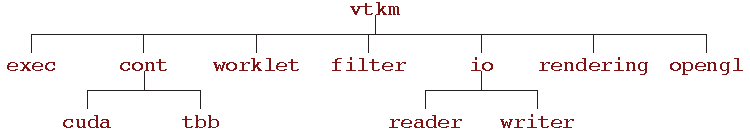
\includegraphics{images/PackageHierarchy}
  \fix{Make a graphic of the package hierarchy.}
  \caption{VTK-m package hierarchy.}
  \label{fig:Packages}
\end{figure}

By convention all classes will be defined in a file with the same name as
the class name (with a \textfilename{.h} extension) located in a directory
corresponding to the package name. For example, the \vtkmcont{ArrayHandle}
class is found in the \vtkmheader{vtkm/cont}{ArrayHandle.h} header. There
are, however, exceptions to this rule. Some smaller classes and types are
grouped together for convenience. These exceptions will be noted as
necessary.

Within each namespace there may also
be \textnamespace{internal}\indexnamespaceone{internal}
and \textnamespace{detail}\indexnamespaceone{detail}
sub-namespaces. The \textnamespace{internal} namespaces contain features
that are used internally and may change without
notice. The \textnamespace{detail} namespaces contain features that are
used by a particular class but must be declared outside of that
class. Users should generally ignore classes in these namespaces.

\index{packages|)}


\section{Function and Method Exports}
\label{sec:FunctionAndMethodExports}

Any function or method defined by VTK-m must come with an export modifier
that determines in which environments the function may be run. These export
modifiers are C macros that VTK-m uses to instruct the compiler for which
architectures to compile each method. Most user code outside of VTK-m need
not use these macros with the important exception of any classes passed to
VTK-m. This occurs when defining new worklets, array containers, and device
adapters.

VTK-m provides three export macros, \vtkmcontexport, \vtkmexecexport, and
\vtkmexeccontexport, which are used to declare functions and methods that
can run in the control environment, export environment, and both
environments, respectively. These macros get defined by including just
about any VTK-m header file, but including \vtkmheader{vtkm}{Types.h} will
ensure they are defined. 

The export macro is place after the template declaration, if there is one,
and before the return type for the function. Here is a simple example of a
function that will square a value. Since most types you would use this
function on have operators in both the control and execution environments,
the function is exported to both places.

\vtkmlisting{Usage of export macro.}{ExportMacro.cxx}

The primary function of the export macros is to interject compiler-specific
keywords that specify what architecture to compile code for. For example,
when compiling with CUDA\index{CUDA}, the control exports have
\textcode{\_\_host\_\_} in them and execution exports have
\textcode{\_\_device\_\_} in them.

There is one additional export macro that is not used for functions but
rather used when declaring a constant data object that is used in the
execution environment. This macro is named
\vtkmmacro{VTKM\_EXEC\_CONSTANT\_EXPORT}\index{export!constant}\index{constant~export}
and is used to declare a constant lookup table used when executing a
worklet. Its primary reason for existing is to add a
\textcode{\_\_constant\_\_} keyword when compiling with CUDA. This export
currently has no effect on any other compiler.


\section{\fix{Remaining Sections}}


\chapter{Provided Worklets}
\label{chap:ProvidedWorklets}

\fix{Write this once some worklets are provided. I expect before this we
  will have a chapter on provided filters. In fact, that probably means
  this chapter should move after the chapters on control and execution
  environments.}

\chapter{Control Environment}
\label{chap:ControlEnvironment}

\fix{Write this.}

\chapter{Execution Environment}
\label{chap:ExecutionEnvironment}

\fix{Write this.}

\chapter{OpenGL Interoperability}
\label{chap:OpenGLInteroperability}

\chapter{Coding Conventions}
\label{chap:CodingConventions}


\begin{flushleft}
  \clearpage
  \lhead[]{}
  \rhead[]{}
  \phantomsection
  \addcontentsline{toc}{chapter}{Index}
  \printindex
\end{flushleft}

\input{Distribution}

\end{document}
